\chapter{Standard LM}\label{chap:standard-lm}

This chapter provides the necessary theoretical foundation to understand general language modeling, without specifically focusing on the code completion task. It begins with the formulation and presents a probabilistic perspective on the models employed to represent language. Subsequently, it explores the transformer architecture and the training of such models. The chapter concludes with a discussion on the inference and sampling processes of trained models.

In this chapter, the term \textit{language} refers to an arbitrary natural language, as opposed to a formal one.

\section{Definition}

Consider a natural language denoted as \(\mathcal{L}\), which is a set of all possible sentences in this language. A sentence \(\bm{x}_{1:T}\) of length \(T\) is a sequence of words \((x_1, x_2, \ldots, x_T)\), where each word is an element of the vocabulary \(V\). Given that some sentences are more likely to occur than others, there exists a joint probability distribution \(P : \mathcal{L} \to [0, 1]\) over variable-length sequences from \(\mathcal{L}\). The model \(p_\theta\) with parameters \(\theta\) (also called weights) that represents this distribution is called a language model, and the task of creating such a model is referred to as language modeling.

Although natural languages are infinite due to their recursive structure, they have a finite number of words, meaning \(K = |V| \in \mathbb{N}\). To demonstrate this, consider that word lengths are finite, which implies that \(\mathcal{L}\) certainly contains a word with the maximum length \(M\). Let the number of characters involved in word formation be \(N\). A very rough upper bound estimate for the number of words in \(\mathcal{L}\) can be calculated using the formula \(N^M\), which is finite because both \(N\) and \(M\) are finite.

The chain rule of probability can be applied to represent \(P\) as follows:
\begin{equation}\label{eq:probability-chain-rule}
    P(\bm{x}_{1:T}) = P(x_1) \cdot P(x_2 \mid x_1) \cdot P(x_3 \mid x_2, x_1) \cdots = \prod_{t=1}^{T}P(x_t \mid \bm{x}_{1:t-1})
\end{equation} 
This indicates that language modeling is equivalent to estimating the probability of each word in the sentence given all the preceding words (i.e., the context), where the probability distribution over each word is a \(K\)-dimensional categorical distribution.

This indicates that language modeling is equivalent to estimating the probability of each word in the sentence given all the preceding words (i.e., the context), where the probability distribution over each word is a \(K\)-dimensional categorical distribution. This sequential prediction process, where each word depends only on the prior subsequence, is called autoregressive (AR) language modeling.

\section{Text Representation}

The proper representation of text is critical to effective language modeling design. Treating text as a sequence of words is natural and intuitive for humans, but not the best choice for machines.

\subsection{Tokens}\label{sec:tokens}

The first reason why words may not be the optimal choice for representing discrete units of text is the out-of-vocabulary (OOV) problem, which refers to the presence of words (or tokens) that are absent from a language model's vocabulary. This challenge arises from the inherently dynamic nature of language, which lacks fixed boundaries. As language evolves, some words become obsolete while new ones emerge. Additionally, the text corpora used for training language models often contain typographical errors and other artifacts of human language.

The second reason is that the language models require statistical information about the co-occurrence of words to capture the semantics of the language. It becomes a problem with rare words whose representations in models lack a learning signal. This phenomenon can be lucidly demonstrated with Zipf's law, which states that in a given corpus, the frequency of any word is inversely proportional to its rank in the frequency table \parencite{estoup1916}. This implies that a small number of words are used very frequently, while the majority are rare. Consequently, language models trained on word-level representations may struggle to learn these infrequent words, leading to poor generalization.

One can propose employing character-level text representation. Although this approach completely resolves the OOV problem, it introduces its own limitations. A small vocabulary necessitates processing longer sequences with smaller semantic representation of its units, which introduces additional computational overhead to internally combine these units to form a more integral semantic representation of text.

Thus, there is a trade-off between the size of the vocabulary and the size of input sequences. Minimizing one leads to an increase in the other. A large vocabulary means that some of its units are used very rarely, and their representations lack a learning signal. A small vocabulary means the utilization of more semantically poor units and a greater computational overhead to process longer sequences.

The optimal balance between character-level and word-level representations is subword chunks, generally called tokens. They offer a greater prospect of granularity in text division, which allows addressing the aforementioned trade-off on a more fine-grained level.

\subsection{Byte Pair Encoding for Tokenization}

The OOV problem persists at the token level. A variety of methods exist to address this issue, with one of the most popular being the byte pair encoding (BPE) algorithm. Originally proposed by \citet{gage1994} as a compression algorithm, it was later adapted by \citet{sennrich2015} for word segmentation with the aim of constructing a vocabulary.

The BPE process begins by initializing the vocabulary with individual characters and a special end-of-word symbol. Words are initially represented as sequences of these characters. Given some corpus of text, the algorithm iteratively identifies the most frequent pair of adjacent symbols and merges them into a new symbol. This process continues until a predefined number of merge operations is reached, resulting in a vocabulary composed of both characters and frequently occurring subword units. After the vocabulary is constructed, the same algorithm can be applied to tokenize the text.

This approach allows for a compact representation of text, reducing the sequence length while maintaining the ability to represent rare and unseen words. By balancing the trade-off between vocabulary size and sequence length, BPE enables language models to efficiently handle the dynamic nature of language, capturing both common and rare linguistic patterns.

\subsection{Embeddings}\label{sec:embeddings}

\begin{sloppypar}
After the text is tokenized, it is represented as a sequence of tokens \((x_1, x_2, \ldots, x_T)\), where \(x_i \in \{1, 2, \ldots, K\}\) is a corresponding integer identifier. A parameterized language model \(p_\theta\) should have the ability to process this sequence of integers. Since most effective models are based on neural networks (NNs), \(\theta\) is a set of matrices that define some non-linear transformation over the continuous vector space. Therefore, tokens need to be embedded into the input vector space \(\mathbb{R}^d\).
\end{sloppypar}

The most straightforward approach is to set \(d=K\) and use one-hot encoding, which assigns a vector \(\mathbf{x}_i = \textrm{one-hot}(x_i) \in \{0, 1\}^K\) full of zeros except for the position corresponding to the token, which is set to one. The resulting vectors capture the identity of the tokens but lack the interaction effects between them.

This issue is resolved by incorporating the first layer of the NN as a trainable embedding matrix \(\mathbf{E} \in \mathbb{R}^{d' \times K}\), which maps each token to a vector \(\mathbf{Ex}_i\) in \(\mathbb{R}^{d'}\), called an embedding, by multiplying its one-hot encoding with \(\mathbf{E}\). Note that the sparse nature of one-hot representations allows this multiplication to be implemented using a lookup table by taking the \(i\)-th column of \(\mathbf{E}\).

There are multiple ways to train the embedding matrix \(\mathbf{E}\). The choice of method depends on the desired properties. In the case of language modeling, the primary requirement is the alignment of the embeddings with the rest of the model weights. Therefore, the embeddings are frequently initialized and trained jointly with the rest of the model parameters.

The trained embeddings capture the semantics of the tokens. This means that tokens occurring in similar contexts tend to have similar embeddings. This phenomenon is known as the distributional hypothesis \parencite{harris1954}. The most common measure of similarity between two embeddings is their dot product or its normalized version, cosine similarity: % TODO: add a figure with king, queen; note it in the text
\begin{equation}
    \cos(\mathbf{x}, \mathbf{y}) = \frac{\mathbf{x}^\top \mathbf{y}}{\|\mathbf{x}\| \|\mathbf{y}\|}.
\end{equation}  

As the dot product suffers from the curse of dimensionality, the number of dimensions \(d'\) required to capture all semantic patterns is exponentially smaller than the vocabulary size \(K\). This is achieved by the fact that two dissimilar vectors do not necessarily have to be orthogonal, as their dot product is already near zero.

\section{Transformer Models}

The most widely used architecture for language modeling is the Transformer model proposed by \citet{vaswani2017}. It is based on the attention mechanism, with its roots introduced by \citet{bahdanau2014}. Since then, a vast number of various architectural modifications have appeared. However, the core idea remains the same.

In the primary source paper, the authors proposed two parts of the architecture: the encoder and the decoder. Both of them, or their combination, are used depending on the specific task. In the case of language modeling (including code modeling), the decoder-only variant has gained widespread adoption. This part of the text describes only this type of Transformer.

\subsection{Overview of the Forward Pass}

Consider the sequence of context tokens \(\bm{x}_{1:t-1} = (x_1, x_2, \ldots, x_{t-1})\) from \equationref{eq:probability-chain-rule}. To model the probability \(p_{\theta}(x_t \mid \bm{x}_{1:t-1})\) of the next token \(x_t\), the decoder-only Transformer first embeds the context tokens into vectors \((\mathbf{Ex}_1, \mathbf{Ex}_2, \ldots, \mathbf{Ex}_{t-1})\) and then passes them through the stack of decoder layers to obtain the contextually enriched embeddings \((\mathbf{h}_1, \mathbf{h}_2, \ldots, \mathbf{h}_{t-1})\), which are called hidden states. It then takes the last hidden state and multiplies it by the weights matrix to get the logits \(\mathbf{z}_t = \mathbf{Wh}_{t-1}\). The \(\mathbf{W}\) is often called the language modeling head. The softmax function is then used to get the parameters of the categorical distribution over the vocabulary:
\begin{equation}\label{eq:softmax}
    \mathbf{p}_t = \mathrm{softmax}(\mathbf{z}_t) = \frac{\exp(\mathbf{z}_t / \tau)}{\sum_{k=1}^{K} \exp(z_{t,k} / \tau)},
\end{equation}
where the exponent in the numerator and division are element-wise functions, and \(\tau\) is a temperature parameter discussed in \sectionref{sec:sampling}.

The resulting vector of estimated probabilities \(\mathbf{p}_t\) can be used in multiple ways. First, to fulfill the original task of language modeling, the element corresponding to the next token \(x_t\) can be extracted from \(\mathbf{p}_t\) and serve as \(p_{\theta}(x_t \mid \bm{x}_{1:t-1})\) in \equationref{eq:probability-chain-rule}. Second, one can sample from the categorical distribution defined by \(\mathbf{p}_t\) to get the next token and thus generate a new sequence from the model, which means that the language model can be used as a generative model. Both settings are commonly used. The first one is employed for the training process, while the second one is used for inference.

Before delving into the specifics of the decoder layer, two important points should be noted. First is that the initial token lacks context. Consequently, a special beginning of sequence (BOS) token is utilized to provide context and serve as an embedding for \(p_\theta(x_1)\). Second, for simplicity, the bias term is omitted in all the weight application formulas, as its inclusion is optional and contingent upon the engineer's design choices.

\subsection{Decoder Layer}

Let's denote the input embeddings as \((\mathbf{x}_1, \mathbf{x}_2, \ldots, \mathbf{x}_{T})\), where \(\mathbf{x}_i \in \mathbb{R}^{d_{\mathrm{model}}}\) for each \(i \in \{1, 2, \ldots, T\}\), and let \(\mathbf{X} \in \mathbb{R}^{T \times d_{\mathrm{model}}}\) represent their concatenated form. The decoder layer then applies the following operations:
\begin{align}
    \mathbf{X}^{(1)} &= \mathbf{X} + \mathrm{MultiHead}(\mathrm{Norm}(\mathbf{X})), \\
    \mathbf{X}^{(2)} &= \mathbf{X}^{(1)} + \mathrm{MLP}(\mathrm{Norm}(\mathbf{X}^{(1)})),
\end{align}
where \(\mathbf{X}^{(2)} \in \mathbb{R}^{T \times d_{\mathrm{model}}}\) is the output of the layer, and \(\mathrm{Norm}\), \(\mathrm{MultiHead}\), \(\mathrm{MLP}\) are sub-layers discussed below.

These formulas differ from the original architecture described in \citet{vaswani2017} as they employ pre-normalization (\cite{baevski2018};~\cite{child2019};~\cite{wang2019}). This modification enhances the stability of the training process by ensuring that the residual embedding stream is modified only through addition, which helps maintain well-behaved gradients at initialization \parencite{xiong2020}. To illustrate this concept in comparison to the original post-normalization structure, \figureref{fig:post-vs-pre-norm} is provided.

\begin{figure}[ht]
    \centering
    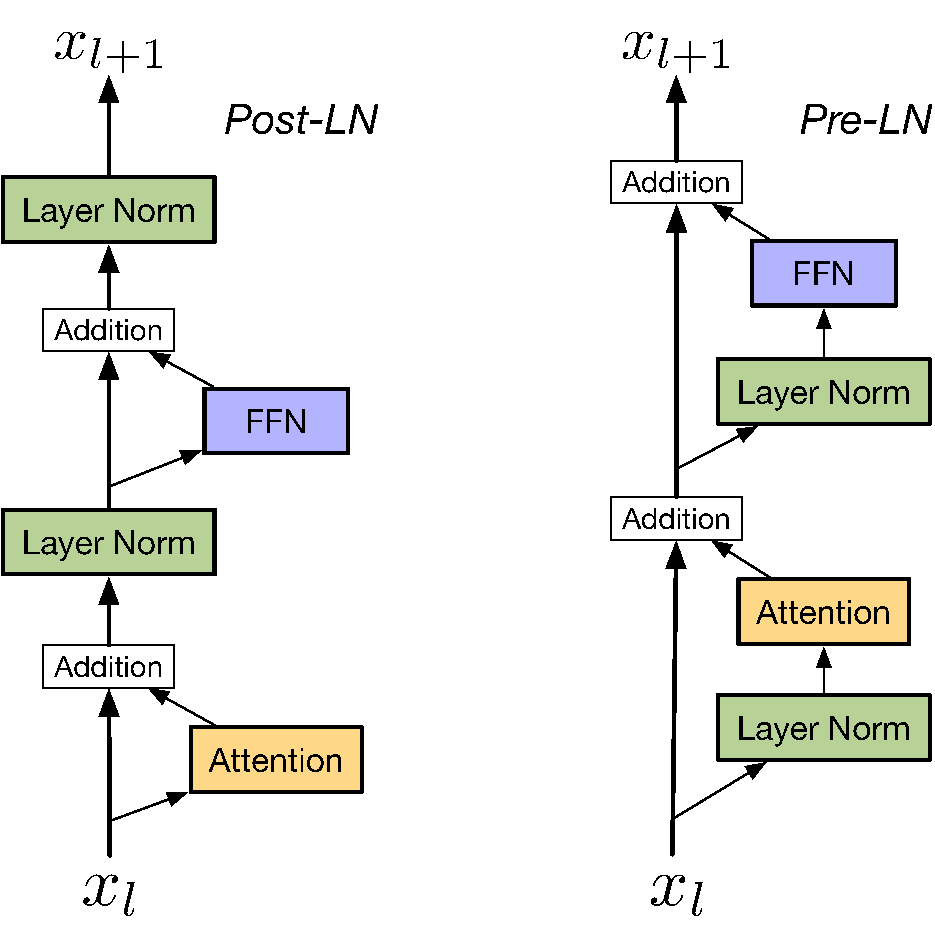
\includegraphics[width=0.7\textwidth]{figures/post-vs-pre-norm.pdf}
    \caption{Comparison of post-normalization and pre-normalization architectures in Transformer models}\label{fig:post-vs-pre-norm}
    \hfill\textit{Source: \citet{ding2021}}
\end{figure}

\subsection{Normalization}

The normalization layer stabilizes the training process by normalizing the input embeddings independently for each token. Various types of normalization layers exist. While the original architecture used layer normalization \parencite{ba2016}, root mean square layer normalization \parencite{zhang2019} has also been widely adopted.

\subsection{Attention}

Consider two additional architectural parameters \(d_k\) and \(d_v = d_{\mathrm{model}}\). The attention layer is described using three weight matrices: \(\mathbf{W}_Q, \mathbf{W}_K \in \mathbb{R}^{d_k \times d_{\mathrm{model}}}\) and \(\mathbf{W}_V \in \mathbb{R}^{d_v \times d_{\mathrm{model}}}\). The output of the layer is calculated as follows:
\begin{equation}\label{eq:attention}
    \mathrm{Attention}(\mathbf{Q}, \mathbf{K}, \mathbf{V}) = \mathrm{softmax}\left(\frac{\left[\mathbf{QK}^\top\right]_{\mathrm{mask}}}{\sqrt{d_k}}\right)\mathbf{V},
\end{equation}
where \(\mathbf{V} = \mathbf{XW}_V^{\top}\) and \(\{\mathbf{Q}, \mathbf{K}\} = \mathrm{RoPE}(\mathbf{XW}_{\{Q, K\}}^\top)\) with \(\mathrm{RoPE}\) denoting the rotary position embedding discussed in \sectionref{sec:rotary-position-embedding}. The softmax is applied row-wise, and \([\ \cdot \ ]_{\mathrm{mask}}\) is a causal masking operation that sets all elements above the main diagonal to \(-\infty\), thereby preventing data leakage from future tokens.

\begin{figure}[ht]
    \centering
    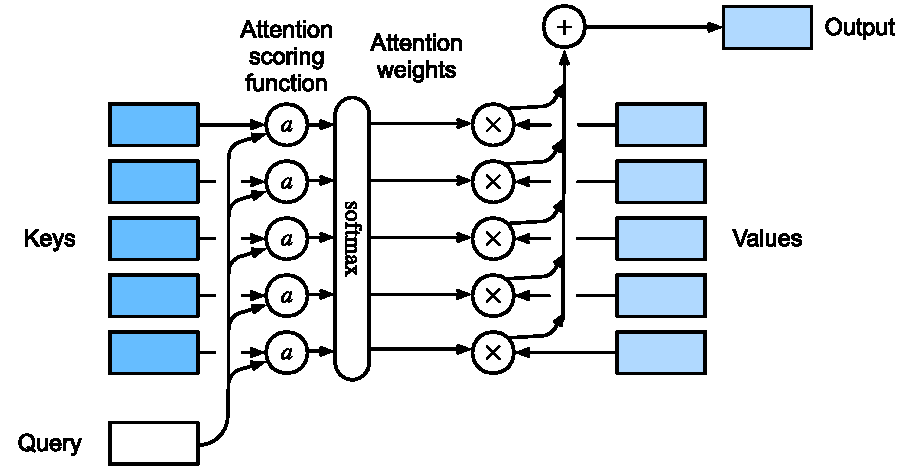
\includegraphics[width=0.85\textwidth]{figures/attention.pdf}
    \caption{Attention mechanism at the single token level}\label{fig:attention}
    \hfill\textit{Source: \citet{zhang2023b}}
\end{figure}

Attention functions as a layer that enables tokens to communicate with each other. Each token performs a query \(\mathbf{q}_i\) to all preceding tokens and itself \(\mathbf{k}_{j \le i}\). The corresponding attention weight of the query-key match \(\mathbf{q}_{i}^\top\mathbf{k}_{j}\) is normalized by the softmax and used as a soft dictionary lookup to retrieve the partial component of the value vector \(\mathbf{v}_j\). The convex combination of all such value vectors \(\mathbf{v}_{j \le i}\) becomes the output of the attention layer. This operational flow for a single query is illustrated in \figureref{fig:attention}.

\subsection{Multi-Head Attention}

Multi-head attention is a modification of the basic attention mechanism. Instead of applying the attention mechanism once, the embedding processing is divided into multiple heads that perform attention in parallel. Given the number of heads \(h\) and an additional output projection weight matrix \(\mathbf{W}_O \in \mathbb{R}^{hd_v \times d_{\mathrm{model}}}\), the output of the layer is calculated as:
\begin{align}
    \mathrm{MultiHead}(\mathbf{X}) &= \\ \mathrm{MultiHead}(\mathbf{Q}, \mathbf{K}, \mathbf{V}) &= \mathrm{Concat}(\mathrm{head}_1, \ldots, \mathrm{head}_h) \mathbf{W}_O \\
    \text{where}~\mathrm{head_i} &= \mathrm{Attention}(\mathbf{Q}_i, \mathbf{K}_i, \mathbf{V}_i),
\end{align}
where \(\mathbf{Q}_i, \mathbf{K}_i, \mathbf{V}_i\) are obtained by applying an independent set of weight matrices \(\mathbf{W}_Q^{(i)}, \mathbf{W}_K^{(i)}, \mathbf{W}_V^{(i)}\) to the input embeddings \(\mathbf{X}\), and \(\mathbf{Q}, \mathbf{K}, \mathbf{V}\) are their concatenated versions.

In this version of the attention, \(d_v\) is not necessarily equal to \(d_{\mathrm{model}}\).

\subsection{Multi-Layer Perceptron}

A multi-layer perceptron (MLP) is a simple feed-forward neural network with two linear transformations and a non-linear activation function. It is applied to each token independently.

Originally, the rectified linear unit (ReLU) was used as the activation function. However, other alternatives have empirically been shown to perform better. Two of these are the Gaussian error linear unit (GELU) and the sigmoid linear unit (SiLU) from \citet{hendrycks2016}. Another is the swish gated linear unit (SwiGLU) introduced in \citet{shazeer2020}.

\subsection{Dropout}

Dropout is a widely adopted regularization technique that enhances the generalization of the model \parencite{srivastava2014}. During the training process, it randomly masks some of the activations of the preceding layer with a probability \(p_{\mathrm{dropout}}\) and scales the remaining activations by a factor of \(1 / p_{\mathrm{dropout}}\) to maintain the output statistics of the layer. This process is conceptually illustrated in~\figureref{fig:dropout}.

\begin{figure}[ht]
    \centering
    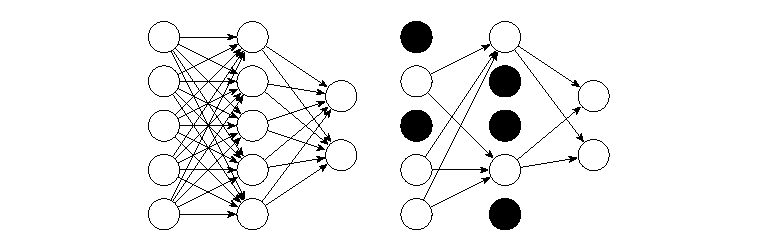
\includegraphics[width=\textwidth]{figures/dropout.pdf}
    \caption{An application of dropout to a multi-layer perceptron}\label{fig:dropout}
    \hfill\textit{Source: \citet{labach2019}}
\end{figure}

This method is frequently applied in transformers across all layers, including the dropout of the attention scores calculated before the application of the softmax function. (\cite{vaswani2017};~\cite{zehui2019})

\subsection{Rotary Position Embedding}\label{sec:rotary-position-embedding}

Rotary Position Embedding (RoPE) is a modification built upon the vanilla Transformer to incorporate the positional information of tokens and address issues present in the originally proposed analogous approach. RoPE was introduced by \citet{su2021} and quickly gained widespread adoption.

For each embedding \(\mathbf{x}_m\) at position \(m\) in the sequence, RoPE proposes a rotation of its query and key vectors:
\begin{equation}
	\{\mathbf{q}_m, \mathbf{k}_m\} = \mathrm{RoPE}(\mathbf{W}_{\{Q, K\}}\mathbf{x}_m, m) = \mathbf{R}^d_{\Theta, m}\mathbf{W}_{\{Q, K\}}\mathbf{x}_m 
\end{equation}
using an orthogonal rotary matrix  
\begin{equation}    
	\mathbf{R}^d_{\Theta,m} = 
	\scalebox{0.8}{\(
	\begin{pmatrix}
		\cos{m\theta_1}& -\sin{m\theta_1}&0&0&\cdots&0&0\\
		\sin{m\theta_1}&\cos{m\theta_1}&0&0&\cdots&0&0 \\
		0&0&\cos{m\theta_2}& -\sin{m\theta_2}&\cdots&0&0\\
		0&0&\sin{m\theta_2}&\cos{m\theta_2}&\cdots&0&0 \\
		\vdots&\vdots&\vdots&\vdots&\ddots&\vdots&\vdots\\
		0&0&0&0&\cdots&\cos{m\theta_{d/2}}& -\sin{m\theta_{d/2}}\\
		0&0&0&0&\cdots&\sin{m\theta_{d/2}}&\cos{m\theta_{d/2}}
	\end{pmatrix}
	\)},
\end{equation}
where \(d = d_k\) and \(\Theta = \{\theta_i=\theta_{\mathrm{base}}^{-2(i-1)/d}, i \in \{1, 2, \ldots, d/2\}\}\) is a predefined set of frequencies derived from the base frequency hyperparameter \(\theta_{\mathrm{base}}\). RoPE can be interpreted as a rotation of two-dimensional scalar chunks of the query and key vectors, determined by both the token's position within the sequence and the chunk's position within the vector, as illustrated in \figureref{fig:rope}.

\begin{figure}[ht]
    \centering
    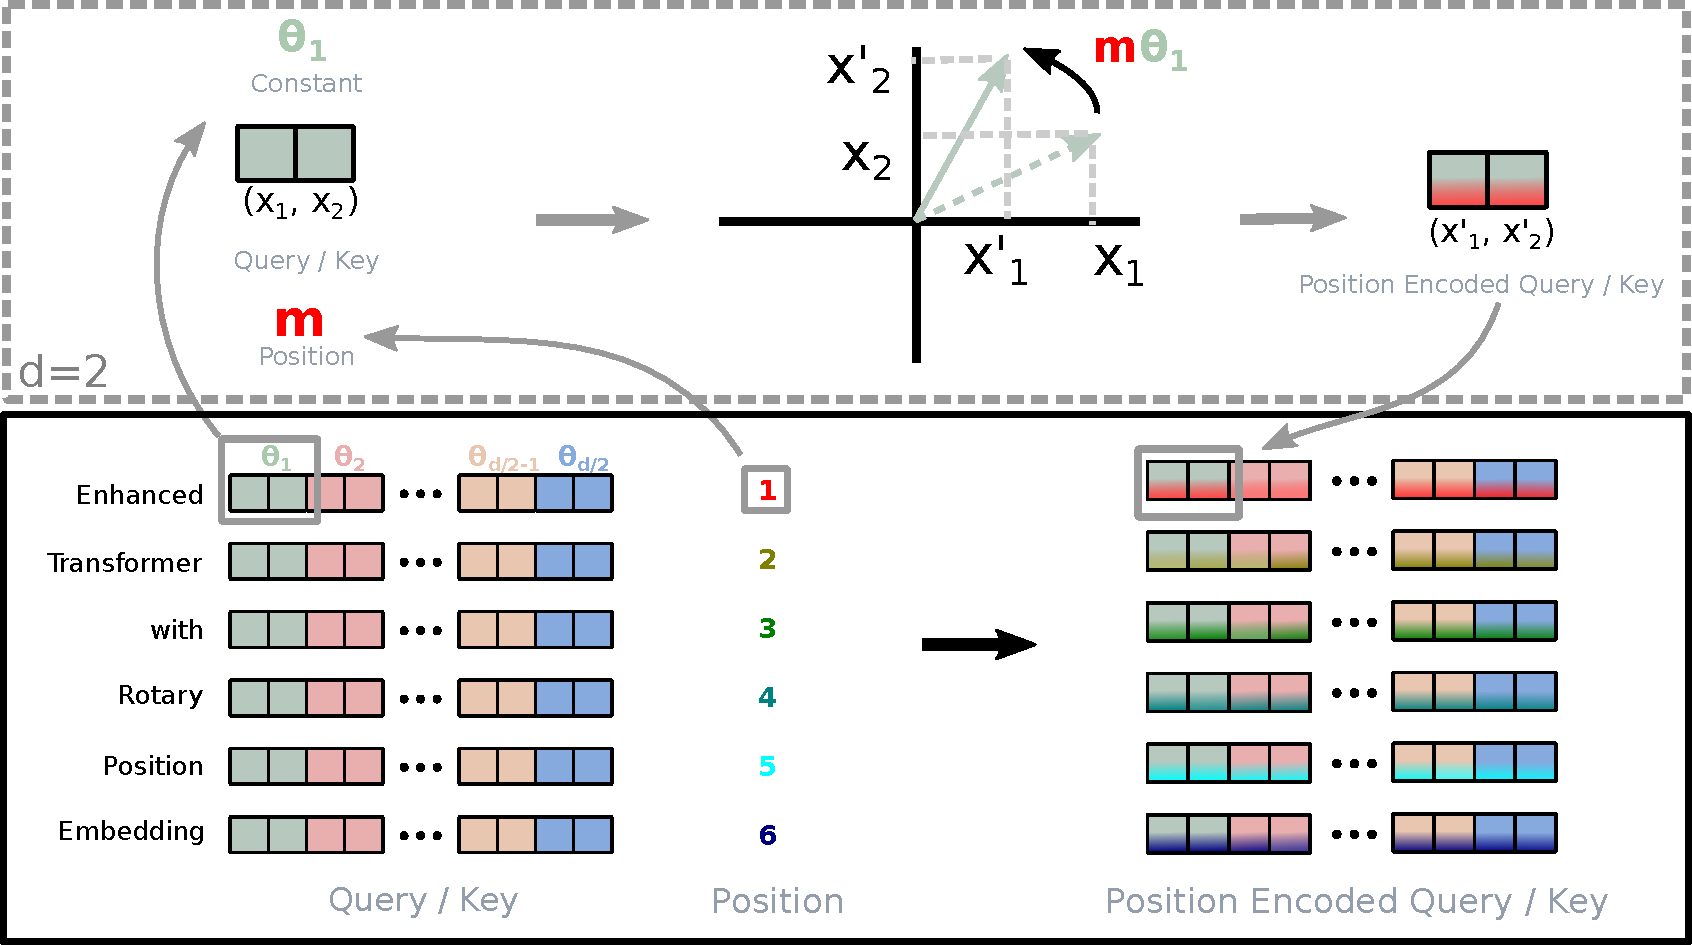
\includegraphics[width=\textwidth]{figures/rope.pdf}
    \caption{Illustration of the effect of RoPE on the query and key vectors}\label{fig:rope}
    \hfill\textit{Source: \citet{su2021}}
\end{figure}

Note two important details regarding the application of RoPE. First, it requires \(d\) to be even. Second, it is applied across all heads in multi-head attention without repeating the rotation frequency \(h\) times, inherently adding more functional bias to heads working on higher frequencies \parencite{barbero2024}.

When multiplying query and key matrices in \equationref{eq:attention}, the two embeddings \(\mathbf{x}_m\) and \(\mathbf{x}_n\) derive the attention score decay based on the relative distance \(m-n\) between them:
\begin{equation}
	\mathbf{q}_m^{\top}\mathbf{k}_n
	=(\mathbf{R}^d_{\Theta, m}\mathbf{W}_Q\mathbf{x}_m)^\top(\mathbf{R}^d_{\Theta, n}\mathbf{W}_K\mathbf{x}_n) =\mathbf{x}_m^\top\mathbf{W}_Q\mathbf{R}^d_{\Theta, n-m}\mathbf{W}_K\mathbf{x}_n,
\end{equation}
which allows the model to capture the positional information of the tokens.

\section{Training}

To elaborate on the process of convergence from a randomly initialized model to one with desirable properties, this section provides an overview of the training process by deriving the direct objective and describing the optimization algorithm, along with associated batch-related terminology and learning rate scheduling.

\subsection{Maximum Likelihood Estimation}

Training the language model \(p_\theta\) involves aligning the distribution it represents with the true data distribution. However, the later is unknown, and only a finite set \(\mathcal{D} = \{\bm{x}^{(1)}, \bm{x}^{(2)}, \ldots, \bm{x}^{(n)}\}\) of instances sampled from it is available. The training objective \(\mathcal{L}_{\mathcal{D}}\), known as the likelihood function, is expressed as the probability of these samples being generated by the model. Assuming that samples are independent and identically distributed, \(\mathcal{L}_{\mathcal{D}}\) can be decomposed into the product of individual probabilities:
\begin{equation}
	\mathcal{L}_{\mathcal{D}}(\theta) = p_{\theta}(\bm{x}^{(1)}, \bm{x}^{(2)}, \ldots, \bm{x}^{(n)}) = \prod_{i=1}^{n} p_{\theta}(\bm{x}^{(i)}) \rightarrow \max.
\end{equation}
The method of estimating the parameters \(\theta\) by maximizing this function is called maximum likelihood estimation (MLE).

Due to several reasons, including underflow issues, the log-likelihood function is often used instead:
\begin{equation}
	\ell_{\mathcal{D}}(\theta) = \log \mathcal{L}_{\mathcal{D}}(\theta) = \log \prod_{i=1}^{n} p_{\theta}(\bm{x}^{(i)}) = \sum_{i=1}^{n} \log p_{\theta}(\bm{x}^{(i)}).
\end{equation}
Optimizing both functions is equivalent, as the logarithm is a monotonically increasing function.

To take one step further, a minus sign can be added to focus on minimization instead of maximization, thereby formulating the negative log-likelihood loss function. Additionally, \equationref{eq:probability-chain-rule} can be used to express the loss function as a sum of the log-likelihoods of the individual tokens:
\begin{equation}
	L(\theta) = -\ell_{\mathcal{D}}(\theta) = -\sum_{i=1}^{n} \sum_{t=1}^{T_i} \log p_{\theta}(x^{(i)}_t \mid \bm{x}^{(i)}_{1:t-1}) \rightarrow \min.
\end{equation}
This objective corresponds to the cross-entropy (CE) loss, which is often represented using the dot product of \(\mathbf{p}^{(i)}_t\) from \equationref{eq:softmax} and the one-hot encoding of the target token \(x^{(i)}_t\).

\subsection{Gradient-Based Optimization}

Various optimization algorithms have been developed to train neural networks. The most effective ones are based on first-order methods, which iteratively adjust the parameters by subtracting the stochastic gradient of the loss function with respect to the parameters. The degree of this adjustment is controlled by multiplicative factor of the gradients called learning rate. Gradients are calculated using a subsample of the training set, known as a mini-batch (or simply batch), with the application of automatic differentiation.

In the field of language modeling, the adaptive moment estimation (Adam) \parencite{kingma2014}, a modification of stochastic gradient descent (SGD), and its version supporting weight decay \parencite{loshchilov2017} are the most popular algorithms. Adam maintains two moving average statistics, called the first and second moments, for each parameter, which correct the application of the gradient and accelerate convergence.

Training is sometimes conducted using a half-precision floating-point format to increase computational speed. However, this approach introduces the risk of underflow for small gradient values. To mitigate this issue, \textit{gradient scaling} is employed. This technique multiplies the loss value by a constant factor, allowing the gradients to maintain appropriate magnitudes during backpropagation. When the optimization step is performed, the gradients are rescaled by the same factor to restore the original learning rate setting. The scaling factor is often determined automatically. \parencite{nvidia2024}

\begin{sloppypar}
Another common modification applied to gradients is \textit{clipping}, which projects the gradient vector onto the surface of a hypersphere with a radius equal to a predefined value if its norm exceeds this threshold. This process prevents gradients from exploding in regions with sharp loss landscapes and stabilizes the training process. \parencite{pascanu2013}
\end{sloppypar}

\subsection{Batch-Related Terminology}

Due to the operational nature of graphics processing units (GPUs), multiple sequences must be organized to have the same length to be processed in parallel. This is achieved by either padding shorter sequences with special tokens or truncating longer ones. The model's scope of visibility is termed the context window, and its size is referred to as the context length.

In some cases, sequences are randomly shuffled, concatenated, and split to form batches without the need for padding or truncation. This technique is known as batch packing.

When hardware constraints limit batch size, gradient accumulation is utilized. Instead of using the entire batch for a single optimization step, it is divided into micro-batches, which are processed sequentially. The parameters are updated only after all the micro-batches have been processed.

\subsection{Learning Rate Scheduling}

Due to the design of Adam, a few iterations at the beginning of training are required to gather sufficient gradient statistics for better moment estimation. This requirement becomes even more critical in the context of the instability associated with Transformers. During this initial phase, using the full learning rate is inadvisable, as it may lead to unstable updates. To mitigate this issue while utilizing all available data, a warm-up period is introduced in the training process. Throughout this period, the learning rate is gradually increased, often linearly, from zero to the desired value over a predefined number of iterations.

After training with high learning rates, the model benefits from smaller parameter updates as it approaches the local optimum and requires more precise adjustments. This is achieved by decaying the learning rate over time.

To summarize, the learning rate, rather than being a constant hyperparameter, has evolved into a function of the iteration index, thereby opening a new dimension for controlling the training process.

\section{Inference}\label{sec:inference}

This section introduces the fundamental concepts related to the inference process of language models, specifically sampling and stopping criteria.

\subsection{Sampling}\label{sec:sampling}

As previously mentioned, a language model represents a probability distribution over the vocabulary given the preceding context. The iterative process of sampling from this distribution and incorporating these new tokens into the model's context is referred to as generation.

Tokens are selected based on their associated probabilities \(\mathbf{p}_t\) from the softmax output, as described in \equationref{eq:softmax}. The temperature parameter modulates the sharpness of this distribution. There are two limiting cases, which are demonstrated in \figureref{fig:softmax-temperature}: First, as \(\tau \to +\infty\), the distribution becomes uniform, with all tokens having an equal probability of being selected. Second, as \(\tau \to 0^+\), the selection becomes deterministic, choosing the most probable token. This is known as greedy decoding and corresponds to the greedy search algorithm in a graph of all possible sequences, where the language model functions as a heuristic.

\begin{figure}[ht]
    \centering
    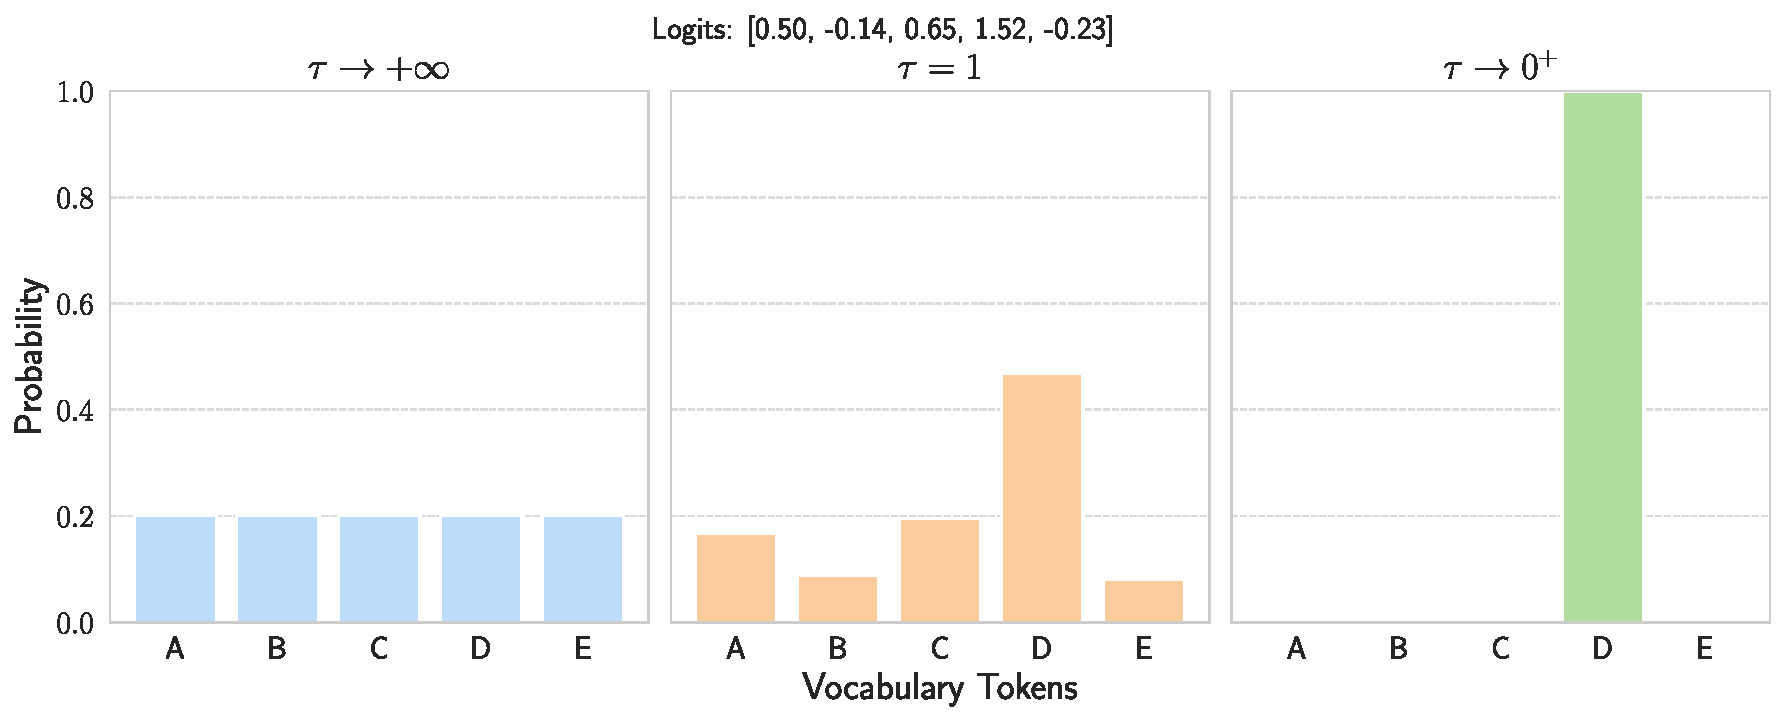
\includegraphics[width=\textwidth]{figures/softmax-temperature.pdf}
    \caption{Impact of the temperature parameter on the softmax output}\label{fig:softmax-temperature}
\end{figure}

To further enhance the quality of the generated text, the top-\(k\) sampling strategy is often employed. It restricts the vocabulary to the top-\(k\) most probable tokens, which helps prevent the model from outputting irrelevant tokens.

A similar concept is applied in the nucleus sampling strategy, also known as top-\(p\) sampling \parencite{holtzman2019}. It restricts the vocabulary to the smallest set of tokens whose cumulative probability exceeds a threshold parameter \(p\).

\subsection{Stopping Criteria}

There are several methods to terminate the generation process.

Firstly, the model can signal the completion of the output sequence by generating an end of sequence (EOS) token. This requires the EOS token to be included in the vocabulary, and the model must be trained to produce it. This is accomplished by appending the EOS token to the end training sequences.

Secondly, algorithmic stopping criteria can be employed. For example, the generation process can be halted when a maximum length threshold is exceeded. Another pertinent example, particularly in the context of code completion, is to cease generation when the model outputs a token containing a newline character.
